\chapter{Z Core Grammatical aspect}
\label{ch:zcga}

The \gls{zcga} is a weak type checker, which checks for grammatical correctness in fully formal Z specifications and partially formalised Z specification. It is not the same as pure Z type checkers as it only checks the grammar on a sentence level and not the logical correctness. The \gls{zcga} has it's roots in weak type theory for mathematics \cite{wtt} and has changed for Z specifications. Core grammatical correctness for Z has also adapted the rules from the \gls{cga} for mathematics (see section \ref{sec:mathlang} in chapter \ref{ch:background}).

This chapter focuses on the first step in the \gls{zmath} approach to translating formal specifcations into theorem provers. The user can check for grammatical correctness with the aim to translate the specification fully into a theorem prover or they can use this step on it's own to check their specification for some sort of correctness.

The first part of this chapter explains the design of the \gls{zcga} and how the rules and categories have been changed. It gives some examples of each of the categories and how they are used in Z. We then explain the rules in which the categories must follow in order to be \gls{zcga} correct. The next section hgihlights some properties we can show about the \gls{zcga}. Then we explain how the categories of the \gls{zcga} syntax are adapted into weak types and check Z specification for correctness.

The final section demonstrates the implementation of the \gls{zcga} and gives examples of certain errors one can get when checking a specification for grammatical correctness.

\section{Weak Types}

Since formal notation is a subset of mathematics we are able to adapt the \gls{cga} for mathematics to work for formal specification and thus the Z notation.

In order to check for grammatical correctness we introduce a weak type system for Z specifications illustrated in figures \ref{tab:zcga1} and \ref{tab:wttrules}.
 
The ZCGa starts from it's lowest level, the \emph{atomic level}, which underlines the elementary characters from which the syntax is made. It then builds itself up to the highest level, \emph{discourse level} where the largest elements can be found. Everything in the \emph{discourse} can be made from
elements in the smaller levels. Everything in the \emph{sentence level} can be made from the levels before and so on.
Types in Z are not the same as weak types. Therefore we shall name each of the weak types, categories to eliminate confusion.

\begin{table}[H]
\begin{tabular}{|l || l | l | c|}
\hline
level & Main category & syntax & Meta-symbol\\
\hline
& \textit{variables} & $V = V ^ {\mathcal{T}} \vert V ^ {\mathbb{S}}$ & x  \\
atomic & \textit{constants} & $C = C ^ {\mathcal{T}} \vert C ^ {\mathbb{S}} \vert C ^ \mathcal{E}$ & c  \\
& \textit{binders} & $B = B ^ {\mathbb{S}} \vert B ^ \mathcal{E}$ & b \\
\hline
phrase & \textit{terms} & $\mathcal{T}$ = $C^{\mathcal{T}}(\overrightarrow{\mathcal{P}})$  $\vert V ^ {\mathcal{T}}$ & t \\
 & \textit{sets} & $\mathbb{S}$ = C$^{\mathbb{S}}(\overrightarrow{\mathcal{P}}$)$\vert B^{\mathbb{S}}_{\mathcal{Z}}(\mathcal{E}) \vert V^\mathbb{S}$ & s \\
\hline
sentence & \textit{expressions} & $\mathcal{E}$ = $C^{\mathcal{E}}(\overrightarrow{\mathcal{P}}) \vert B^{\mathcal{E}}_{\mathcal{Z}}(\mathcal{E})$ & E  \\
& \textit{definitions} & $\mathcal{D} = C^{\mathbb{S}}(\overrightarrow{V}):= \mathbb{S}$ & D \\
\hline
discourse & \textit{schematext} & $\mathbf{\Gamma}$ = $\emptyset \vert \mathbf{\Gamma}, \mathcal{Z} \vert \mathbf{\Gamma}, \mathcal{E}$ & $\Gamma$\\
& \textit{paragraphs} & $\Theta$ = $\mathbf{\Gamma} \triangleright \mathcal{E} \vert \mathbf{\Gamma} \triangleright \mathcal{D}$ & $\theta$\\
& \textit{specifications} & \textbf{Spec} = $\emptyset \vert \mathbf{Spec}, \Theta$  & spec \\
\hline
\end{tabular}

\begin{tabular}{|l|l|c|}
\hline
Other Category & abstract syntax & Meta-symbol\\
\hline
\textit{parameters} & $\mathcal{P} = \mathcal{T} \vert \mathbb{S} \vert \mathcal{E}$ & P\\
\textit{declarations} & $\mathcal{Z}$ = V$^{\mathbb{S}}$:SET $\vert$ V$^{\mathcal{T}}$:$\mathbb{S}$ & Z\\
\hline
\end{tabular}

Note:
$\overrightarrow{\mathcal{P}}$ is a list of 0 or more $\mathcal{P}$'s, $\overrightarrow{\mathbb{S}}$ is a list of 0 or more $\mathbb{S}'s$,\\
$\overrightarrow{\mathcal{E}}$ is a list of 1 or more $\mathcal{E}'s$, $\overrightarrow{V}$ is a list of 0 or more $V's$.
\caption{Categories of ZCGa syntax.} \label{tab:zcga1}
\end{table}

These categories are adapted from the weak types in \cite{wtt}. In particular \emph{book} becomes \emph{specification}, \emph{lines} become \emph{paragraphs}, \emph{context} becomes \emph{schematext} and \emph{statements} become \emph{expressions}. We eliminate \emph{nouns}, \emph{adjectives} and only have one syntax for \emph{definition}.

\subsection{Examples of specifications and weak types}
Everything within a Z specification can be labelled using the categories found in table \ref{tab:zcga1}.

\begin{figure}[H]
\centering
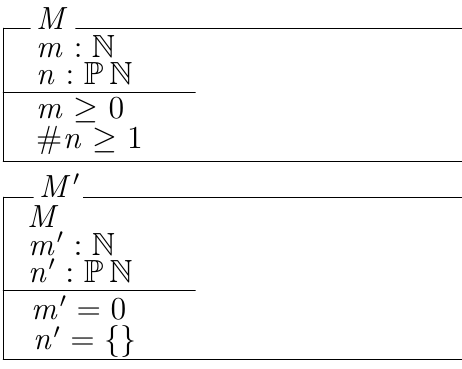
\includegraphics[scale=0.4]{Figures/zcga/toy.png}
\caption{Basic example of a specification \label{fig:toy}}
\end{figure}

Using figure \ref{fig:toy} we will give examples of individual weak type categories.

\paragraph{variables}
\label{subsubsec:variables}

The set of variables $V$ is divided into two subsets $V^{\mathcal{T}}\text{ and } V^{\mathbb{S}}$ which correspond to variables giving terms and variables giving sets respectively.

\begin{itemize}
\item $V^{\mathcal{T}}$. An example of a variable giving a term would be `$m$' in figure \ref{fig:toy}.

\item $V^{\mathbb{S}}$. An example of a variable giving a set would be `$n$' in figure \ref{fig:toy}.
\end{itemize}

\paragraph{constants}
\label{subsubsec:costants}

The set of constants range over constants giving terms $C^{\mathcal{T}}$, constants giving sets $C^{\mathbb{S}}$ and constants giving expressions $C^{\mathcal{E}}$.

\begin{itemize} 
\item $C^{\mathcal{T}}$. An example of a constant giving an expression would be `$0$' in figure \ref{fig:toy}.

\item $C^{\mathbb{S}}$. An example of a constant giving an expression would be `$\{\}$' in figure \ref{fig:toy}.

\item $C^{\mathcal{E}}$. An example of a constant giving an expression would be `$m' = 0$' where the constants is `$=$' from figure \ref{fig:toy}.
\end{itemize}

\paragraph{binders}
\label{subsubsec:binders}

There are two subsets of binders in the categories for Z specifications. Binders giving sets $B^{\mathbb{S}}$, and binders giving expressions $B^{\mathcal{E}}$.

\begin{itemize}
\item $B^{\mathbb{S}}$. An example of a binder giving an expression is 
\newline
\noindent `$\exists schedule:TIMESLOT \leftrightarrow ROOM \bullet (allPairs moduleTT \cap schedule = \emptyset
\land moduleTT = moduleTT \oplus {m? \mapsto schedule})$'
\newline
\noindent taken from Timetable specification in appendix \ref{app:timetable}.

\item $B^{\mathcal{E}}$. An example of a binder giving a set is
\newline
\noindent `$\bigcup \{s:\dom studentTT \bullet \{s \mapsto (studentTT~s \setminus moduleTT~m?)\}$' \newline
\noindent taken from Timetable specification in appendix \ref{app:timetable}.
\end{itemize}

\paragraph{terms}
\label{subsubsec:terms}

Terms can range over constants giving terms with optional parameters $C^{\mathcal{T}}(\overrightarrow{\mathcal{P}})$, and variables giving terms $V^{\mathcal{T}}$.

\begin{itemize}
\item $C^{\mathcal{T}}(\overrightarrow{\mathcal{P}})$. An example of a constant giving a term is `$\# n$' (taken from figure \ref{fig:toy}) the constant being $\#$ which would be in the preface of constants with the weak typing as $\mathbb{S} \rightarrow \mathcal{T}$ and the parameter of this constant giving a term would be `$n$' which is set.

\item $V^{\mathcal{T}}$. See section \ref{subsubsec:variables} on variables giving terms.
\end{itemize}

\paragraph{sets}
\label{subsubsec:sets}

The category of \emph{set} has three sub categories, constants giving sets with optional parameters $C^{\mathbb{S}}(\overrightarrow{\mathcal{P}})$, binders giving sets with expression as its parameter $B^{\mathbb{S}}_{\mathcal{Z}}(\mathcal{E})$ and variables giving sets $V^{\mathbb{S}}$.

\begin{itemize}
\item $C^{\mathbb{S}}(\overrightarrow{\mathcal{P}})$. An example of a constant giving a set with parameters is
\newline
`$studentTT = studentTT \union {s? \mapsto \emptyset}$'
\newline
taken from Timetable specification in appendix \ref{app:timetable}. Where the constant giving a set is `$\union$' and the parameters it takes is `$studentTT$' and `${s? \mapsto \emptyset}$'.

\item $B^{\mathbb{S}}_{\mathcal{Z}}(\mathcal{E})$. An example of a binder giving a set with an expression and declaration as parameters is
\newline

`$\bigcup \{s:\dom studentTT \bullet \{s \mapsto (studentTT~s \setminus moduleTT~m?)\}\}$' \newline
taken from Timetable specification in appendix \ref{app:timetable}. Where the constant is `$\bigcup$', the declaration parameter is `$s:\dom studentTT $' and the expression parameter is `$  \{s \mapsto (studentTT~s \setminus moduleTT~m?)\}$'.

\item $V^{\mathbb{S}}$. See section \ref{subsubsec:variables} on variables giving sets.
\end{itemize}

\paragraph{expressions}
\label{subsubsec:expressions}

The category of expressions ranges over two subsets, constants giving expressions with optional parameteres $C^{\mathcal{E}}(\overrightarrow{\mathcal{P}})$, and binders giving expressions with a declarations and expression $B^{\mathcal{E}}_{\mathcal{Z}}(\mathcal{E})$.

\begin{itemize}
\item $C^{\mathcal{E}}(\overrightarrow{\mathcal{P}})$. A constant giving an expression can be seen in figure \ref{fig:toy} as `$m \geq 0$' where `$\geq$' is the constant giving an expression and the paramters are two terms: `$m$' and `$0$'.

\item $B^{\mathcal{E}}_{\mathcal{Z}}(\mathcal{E})$. A binder giving an expression could be a `$\forall$' or `$\exists$' binder. An example of this is shown in the Timetable specification in appendix \ref{app:timetable} as
\newline
`$\exists schedule : TIMESLOT \leftrightarrow ROOM \bullet(allPairs moduleTT \cap
schedule = \emptyset \land moduleTT = moduleTT \oplus \{m? \mapsto schedule\})$'
\newline
where the binder giving an expression is `$\exists$', the declaration paramter is `$TIMESLOT \leftrightarrow ROOM$' and the binding expression is `$(allPairs moduleTT \cap
schedule = \emptyset \land moduleTT = moduleTT \oplus \{m? \mapsto schedule\})$'.
\end{itemize}

\paragraph{definitions}
\label{subsubsec:definitions}

Theres is only one kind of definition in the weak type theory syntax for Z. A local definition in Z is a constant giving a definitions taking variables as paramters giving a set, $C^{\mathbb{S}}(\overrightarrow{V}):= \mathbb{S}$. An example of this is shown the GenDB specification in appendix \ref{app:gendb}. The definition is
\newline
 `$\mathbf{let}\ cosrel==(parent^{nth?+1}\comp(parent^{-1})^{nth?+1+rem?})\setminus (parent \comp parent^{-1}) \bullet$\newline
\indent $cousins! = cosrel \limg \{p?\}\rimg \union cosrel^{-1} \limg \{p?\} \rimg$'
\newline
where the defined constant is $cosrel$.

\paragraph{schematext}
\label{subsubsec:schematext}

The schematext within a Z specification reighns over three sub categories, either the schema text can be empty $\emptyset$, or it can be schematext with a declaration $\mathbf{\Gamma}, \mathcal{Z}$ or it can be schematext with an expression $\mathbf{\Gamma}, \mathcal{E}$.

\begin{itemize}
\item $\emptyset$. The empty schema text is the beginning of a specification where we start with nothing.

\item $\mathbf{\Gamma}, \mathcal{Z}$. The first declaration in a specification would be the empty $\Gamma$ plus the declaration. For example in figure \ref{fig:toy} the first example of this would be `$m:\nat$', which is the empty schematext $\emptyset$ along with the first declaration of the specification. The second declaration add to the schema text would be $n:\power \nat$ and so on.

\item $\mathbf{\Gamma}, \mathcal{E}$. This set represents all the expressions which are added to the schema text. In the example in figure \ref{fig:toy} we would already have two declarations in the schematext $m:\nat$ and $n:\power \nat$ in the schema text before the first expression is added $m \geq 0$. The second expression added to the schematext in the same example would be $\# n \geq 1$. 

\end{itemize}

\paragraph{paragraphs}
\label{subsubsec:paragraphs}

A paragraph $\Theta$ contains either an expression $\mathbf{\Gamma} \triangleright \mathcal{E}$ or a definition $\mathbf{\Gamma} \triangleright \mathcal{D}$, relative to a schematext.

The symbol $\triangleright$ is a sepatation marker betwen the schematext and expression or definition

\begin{itemize}
\item $\mathbf{\Gamma} \triangleright \mathcal{E}$. Examples of expressions in a paragraph see section \ref{subsubsec:expressions}.

\item $\mathbf{\Gamma} \triangleright \mathcal{D}$. Example of definitions in a paragraph see section \ref{subsubsec:definitions}.
\end{itemize}

\paragraph{specifications}
A specifiation $spec$ is a list of paragraphs: $spec= \emptyset \vert \mathbf{Spec}, \Theta$.

A simple example of a specification is the entire of figure \ref{fig:toy}.

\paragraph{other categories}

Here we describe the other categories which are needed in the \gls{zcga} abstract syntax.

\paragraph{Declarations.} A declaration ina schematext represents the \emph{introduction of a vairable} of a known type. In the categories of ZCGa syntax we can have two different kinds of declarations. This can be: \texttt{SET} (the type of all sets) or a set. Both of these declarations relates a \emph{subject} (the left hand side of the declaration) with its \emph{type/predicate} (right hand side of the declarations). The abstract syntax for the two categories of declarations are $V^{\mathbb{S}}$ is a set  $V^{\mathbb{S}}:SET$, or term $V^{\mathcal{T}}$ is in the set $\mathbb{S}$, $V^{\mathcal{T}:\mathbb{S}}$.

\begin{itemize}
\item$V^{\mathbb{S}}:SET$. An example of this kind of declaration is `$n':\power \nat$' taken from figure \ref{fig:toy}.

\item $V^{\mathcal{T}:\mathbb{S}}$. An example of this kind of declaration is `$m:\nat$' taken from figure \ref{fig:toy}.
\end{itemize}

\paragraph{Parameters.} The list of paramters represent the categories in which constants may depend. The paramters available in the \gls{zcga} abstract syntax are terms $\mathcal{T}$, sets $\mathbb{S}$ or expressions $\mathcal{E}$. For details on how each of these parameters are formed see the relevent sections (\ref{subsubsec:terms}, \ref{subsubsec:sets} and \ref{subsubsec:expressions} respectively).

\subsection{Weak Typing Rules}

The ZCGa uses the weak types found in table \ref{tab:zcga1} and checks the specification is correct according to the rules found in \ref{tab:wttrules}. To write the rules for the \gls{zcga} we must first establish some definitions. The following definitions have been adapted from \cite{wtt} to accomadate Z specifications.

\begin{defin}
We abbreviate $\vdash$ spec $\mathbf{::Spec}$, spec $\vdash \Gamma \mathbf{::\Gamma}$ as OK(spec; $\Gamma$)
\end{defin}

\begin{defin} The set dvar is the set of declared variables in the \emph{schematext} $\Gamma$:
\begin{itemize}
\item If $\Gamma = \emptyset$, then $dvar(\Gamma) = \emptyset$.
\item If $\Gamma' = \Gamma, x:A$ and $x \notin dvar(\Gamma)$, then $dvar(\Gamma') = dvar(\Gamma), x$.
\item Else if $\Gamma' =\Gamma,S,$ then $dvar(\Gamma') = dvar(\Gamma)$.
\end{itemize}
\end{defin}

\begin{defin} We denote a preface for a Z specification spec by prefcons(spec) \footnote{The full set of $prefcons$ can be found in the implementation of the \gls{zcga} checker. They are in under the variable $preface\_constants$.}. This set contains all the constants listed in the preface. If $c \in prefcons(spec)$ and if $K_{1},...,K_{n}$ is the set of the weak types of the parameters of $c$ and if $k$ is the resulting weak type of the full construct $c(...)$, then we attatch the type $k_{1} \times ... \times k_{n} \rightarrow l$ to $c$.
\end{defin}

\begin{exam}

\end{exam} An example of a preface for a Z specification is shown in the following:

\begin{tabular}{| c | c || c | c |}
\hline
constant name & weak type & constant name & weak type \\
\hline
$\nat$ & $\mathbb{S}$ 
& $<$ & $\mathcal{T} \times \mathcal{T} \rightarrow \mathcal{E}$ \\
$-$ & $\mathcal{T} \times \mathcal{T} \rightarrow \mathcal{T}$ 
& $\union$ & $\mathbb{S} \times \mathbb{S} \rightarrow \mathbb{S} $ \\
\hline
\end{tabular}

\begin{defin} We denote a set containing all the constants to be defined in a specification spec by defcons(spec). Let $\Theta \in spec$ be a paragraph containing a definition $\Gamma \triangleright \mathcal{D}$ where $\mathcal{D}$ is in the form $c(x_{1},...,c_{n}):=A$. Then the defined constant of the definition, or $defcons(\mathcal{D})$, is $c$.
\end{defin}


\begin{table}[H]
\begin{tabular}{| c | c | } \hline 
(var) & $\dfrac{OK(spec;\Gamma), x \in V^{\mathcal{T}/\mathbb{S}}, x \in dvar(\Gamma)}{spec;\Gamma \vdash x \mathbf{::}\mathcal{T}/\mathbb{S}}$ 
\\[0.25cm] \hline
(int-cons) & $\dfrac{\begin{aligned}
OK(spec;\Gamma), \Gamma' \rres \mathcal{D} \in spec, \\[0.0001em]
dvar(\Gamma')=\{x_{1}, ..., x_{n}\}, defcons(\mathcal{D}) = c \in C^{\mathcal{T}/\mathbb{S}/\mathcal{E}}, \\
wt_{spec;\Gamma}(P_{i})=wt_{spec;\Gamma'}(x_{i}),\text{ for all }i = 1, ..., n
\end{aligned}}%
{spec;\Gamma \vdash c(P_{1}, ..., P_{n})::\mathcal{T}/\mathbb{S}/\mathcal{E}}$
\\[0.25cm] \hline
(ext-cons) & $\dfrac{\begin{aligned}
OK(spec;\Gamma), c \text{ external to spec}, c \mathbf{::} k_{1} \times... \times k_{n} \rightarrow k, \\
spec;\Gamma \vdash P_{i} \mathbf{::} k_{i} (i=1,...,n)
\end{aligned}}%
{spec;\Gamma \vdash c(P_{1},...,P_{n}) \mathbf{::}k}$ 
\\[0.25cm] \hline
(bind) & $\dfrac{OK(spec;\Gamma;Z), b \in B, b \mathbf{::}k_{1}\rightarrow k_{2}, spec;\Gamma, Z \vdash E \mathbf{::}k_{1}}{spec;\Gamma \vdash b_{z}(E)\mathbf{::}k_{2}}$ 
\\[0.25cm] \hline
(defin)& $\dfrac{\begin{aligned}
spec;\Gamma \vdash s \mathbf{::} \mathbb{S} \\
dvar(\Gamma)=\{x_{1},...,x_{n}\}, c \in C^{\mathbb{S}}, c \notin prefcons(spec) \cup defcons(spec)
\end{aligned}}%
{spec;\Gamma \vdash c(x_{1},...,x_{n}):= s \mathbf{::} \mathcal{D}}$ 
\\[0.25cm] \hline
& $\dfrac{\vdash spec \mathbf{:: Spec}}{spec \vdash \emptyset \mathbf{:: \Gamma}}(emp-cont)$ 
\\[0.25cm] \hline
(set-dec) & $\dfrac{OK(spec;\Gamma), x \in V^{\mathbb{S}}, x \notin dvar(\Gamma)}{spec \vdash \Gamma, x:SET \mathbf{:: \Gamma}}$
\\[0.25cm] \hline
(term-dec) & $\dfrac{OK(spec;\Gamma), spec;\Gamma \vdash s \mathbf{::} \mathbb{S}, x \in V^{\mathcal{T}}, x \notin dvar(\Gamma)}{spec \vdash \Gamma, x:s \mathbf{:: \Gamma}}$ 
\\[0.25cm] \hline
(assump) & $\dfrac{OK(spec;\Gamma), spec;\Gamma \vdash e\mathbf{::}\mathcal{E}}{spec \vdash \Gamma, e \mathbf{:: \Gamma}}$ 
\\[0.25cm] \hline
(emp-spec) & $\dfrac{ }{\vdash \emptyset \mathbf{:: Spec}}$ 
\\[0.25cm] \hline
(spec-ext) & $\dfrac{spec \vdash \Gamma \mathbf{:: \Gamma}}{\vdash spec, \Gamma \mathbf{:: Spec}}$ 
\\[0.25cm] \hline
\end{tabular}
\caption{Weak typing rules used by the ZCGa type checker. \label{tab:wttrules}}
\end{table} 

\subsection{Weak typing properties and definitions}

Since the categories and rules of the Z syntax $WT_{Z}$ are a subset of the original MathLang $WT_{M}$ \cite{wtt}, the following lemma holds:

\begin{lemma}
ZCGa properties \\

\begin{enumerate}
\item Types are unique. I.e.\ if $spec, \Gamma \vdash E \mathbf{::} W$ then $W$ is unique.

\item Type finding is decidable.\ I.e. for any $spec, \Gamma, E$, we can decide if there is $W$/ $spec, \Gamma \vdash E \mathbf{::}W$.

\item Type checking is decidable. I.e. for $spec, \Gamma, E, W$ then we can decide if $spec, \Gamma \vdash E \mathbf{::}W$.
\end{enumerate}
\end{lemma}



\subsection{Adapting weak types to the ZCGa}

For our \gls{zcga} checker we take the core categories from table \ref{tab:wttrules}.

We use 7 categories, \textbf{Spec}, $\mathbf{\Gamma}$, $\mathcal{T}, \mathbb{S}, \mathcal{Z}, \mathcal{E}, \mathcal{D} $ corresponding to \textit{specification}, \textit{schematext}, \textit{term}, \textit{set}, \textit{declaration}, \textit{expression}, and \textit{definition} respectively.
These categories and weak typing rules will aid us to translate a specification into a full proof as they help us complete the GPSa (see Figure \ref{fig:steps}).

\section{Annotations}

Using the ZMathLang \LaTeX{} package the user can label the specification with \gls{zcga} annotations. This can be either before or after labelling the specification with \gls{zdra} (see chapter \ref{chap:zdra}). The \gls{zcga} annotations will highlight each individual grammatical aspect of the specification. Table \ref{tab:zcgannot} shows how to label specifications with \gls{zcga}.

\begin{table}[H]
\begin{tabular}{| l | l | l |}
\hline
\textbf{Category} & \textbf{\LaTeX{} label} & \textbf{Colour} \\
\hline
\hline
Specification & \verb|\specification{...}| & \specification{} \\
SchemaText & \verb|\text{...}| & \cgatext{} \\
Term & \verb|\term{...}| & \term{} \\
Set & \verb|\set{...}| & \set{} \\
Declaration & \verb|\declaration{...}| & \declaration{} \\
Expression & \verb|\expression{...}| & \expression{} \\
Definition & \verb|\definition{...}| & \definition{} \\
\hline
\end{tabular}
\caption{ZCGa \LaTeX{} annotations and their colours. \label{tab:zcgannot}}
\end{table}

\subsection{term}

According to the rules in table \ref{tab:wttrules} for an element to be a well typed term it can be  a variable being declared such as \emph{t} (labelled in blue) in figure \ref{fig:decinzcga} or it can be a constant giving a term. The latter kind of term must have a constant within the preface of constants and a variable which has been declared. An example of this could be the term `\verb|# s|' (shown in figure \ref{fig:consterm}).

\begin{figure}[H]
\centering
\begin{tabular}{|c | c|}
\hline
\verb|\term{\# \set{s}}| &
\term{\# \set{s}} \\
\hline
\end{tabular}
\caption{Constant giving a term \label{fig:consterm}}
\end{figure}

Figure \ref{fig:consterm} shows a constant giving a term. Provided that the set \emph{s} is in the set of declared variable then the term \verb|# s| is a correctly typed term.

\subsection{set}

Similar to typing a term, set can be correctly type in one of two ways. The first is a variable set which is correctly declared such as `\emph{s}' in figure \ref{fig:sdecinzcga}. The second way a set could be correctly typed is by having a constant with parameters.

\begin{figure}[H]
\centering
\begin{tabular}{|c | c|}
\hline
\verb|\set{\set{s} \cup \set{s'}}| &
\set{\set{s} \cup \set{s'}} \\
\hline
\end{tabular}
\caption{Constant giving a term \label{fig:consset}}
\end{figure}

Figure \ref{fig:consset} shows an example of a correctly typed set, consisting of a constant and in this case two parameters (s and s'). So long as s and s' are in the set of declared variables then `\emph{$s \cup s'$}' is a correctly typed set.


\subsection{declaration}

There are two types of grammatically correct declaration:
\begin{enumerate}
\item term declaration
\item set declaration
\end{enumerate}

A term declaration is any declaration, expressing the relation between something and it's type. For example if we had the declaration \verb|t: \nat| this is declaring t is of type some sort of natural number. We can label this declaration in \gls{zcga} (shown in figure \ref{fig:decinzcga})

\begin{figure}[H]
\centering
\begin{tabular}{|c | c|}
\hline
\verb|\declaration{\term{t}: \expression{\nat}}| &
\declaration{\term{t}: \expression{\nat}} \\
\hline
\end{tabular}
\caption{Correct term declaration labelled in zcga \label{fig:decinzcga}}
\end{figure}

We label \emph{$\nat$} as declarations for the same reasons as the typing's behaviour in \cite{wtt}.

The second type of declaration would be the declaration of a set, for example \verb|s: \power \nat| this is saying that the set \emph{s} is in the set \emph{$\power \nat$}. Figure \ref{fig:sdecinzcga} shows how this kind of declaration would be labelled in \gls{zcga}

\begin{figure}[H]
\centering
\begin{tabular}{|c | c|}
\hline
\verb|\declaration{\set{s}: \expression{\power \nat}}| &
\declaration{\set{s}: \expression{\power \nat}} \\
\hline
\end{tabular}
\caption{Correct set declaration labelled in zcga \label{fig:sdecinzcga}}
\end{figure}

\subsection{expression}

An expression (named assump in the rules) is any correct expression within the context. The expression can only contain correct sets and terms in the context. Any constants within the expression must be in the preface of the \gls{zcga} checker. A correct expression is shown in figure \ref{fig:expinzcga}.

\begin{figure}[H]
\centering
\begin{tabular}{|c | c|}
\hline
\verb|\expression{\term{t} \in \set{s}}| &
\expression{\term{t} \in \set{s}}\\
\hline
\end{tabular}
\caption{Correct expression labelled in zcga \label{fig:expinzcga}}
\end{figure}

\subsection{definition}

If all the variables within the definition have been declared and the constant the user is defining is a constant set. As well as the constant the user is defining is not already in predefined and preface constants then the definition is correct. A correct Z definition is shown in figure \ref{fig:definzcga}.

\begin{figure}[H]
\begin{footnotesize}
\centering
\begin{tabular}{|l|}
\hline
\verb|\definition{\LET \set{old} == \set{new} @ \expression{\term{t} \in \set{old}}}| \\
\hline
\definition{\LET \set{old} == \set{new} @ \expression{\term{t} \in \set{old}}}\\
\hline
\end{tabular}
\end{footnotesize}
\caption{Correct definition labelled in zcga \label{fig:definzcga}}
\end{figure}

\subsection{schematext}

Schematext is all the correct declarations, expressions and definitions within a specification. Figure \ref{fig:stinzcga} shows schematext which is correct. The declaration and expression within the content of the schema would be classified as schematext.

\begin{figure}[H]
\centering
\begin{minipage}{0.45\textwidth}
\begin{BVerbatim}
\begin{schema}{K}
\text{\declaration{\set{s}:
\expression{\power \nat}}}
\where
\text{\expression{\term{t} \in \set{s}}}
\end{schema}
\end{BVerbatim}
\end{minipage}\hfill
\begin{minipage}{0.45\textwidth}
\begin{schema}{K}
\cgatext{\declaration{\set{s}: \expression{\power \nat}} }
\where
\cgatext{\expression{\term{t} \in \set{s}}}
\end{schema}
\end{minipage}
\caption{Example of correct schematext \label{fig:stinzcga}}
\end{figure}

\subsection{specification}

Specifications are correct when the schematext is empty or all the schematext within a specification is correct. A full example of a correctly labeled specification in \gls{zcga} is shown in chapter \ref{ch:fullexample} in figure \ref{fig:zcgaschemaout}.

\section{Implementation}

The \gls{zcga} program automtically checks the specification for grammatical correctness. To do this it uses the \gls{zcga} annotions inputted by the user and will notify the user if all is correct or any errors it may encounter. The \gls{zcga} checker is a weak type checker. Therefore it only checks the correctness of the weak types of the specification (annotated) and not actual Z types like a Z type checker would find, such as fuzz.

\subsection{Checking if a specification is ZCGa correct}

The \gls{zcga} program uses regular expressions to read the annotations written by the user to determine with a specification is \gls{zcga} correct. It ignores all the parts which are not labelled in \gls{zcga} which allows for \gls{semiform} to be checked as well. Look at the following:

\begin{exam}
\begin{verbatim}
There is a variable t which is a number that:
\text{\expression{\term{j} < \term{k}}}
\end{verbatim}
\end{exam}

This example shows a small specification that is \gls{semiform}, the \gls{zcga} will read the annotations \verb|\text|, \verb|\expression| and \verb|\term|. It will see that the specification contains a correct expression, however the specification is \gls{zcga} incorrect as it would not pick up that the terms have been declared. For this example to be \gls{zcga} correct the user will need to change it into the example shown in \ref{Kexam}.

If the specification is correctly labelled and follows all the rules in table \ref{tab:wttrules} then a message would appear saying \texttt{Spec Grammatically Correct}. However if the specification is \gls{zcga} incorrect then a message will appear saying `\texttt{Spec Grammatically Incorrect, Number of errors:\emph{n}}' where \texttt{\emph{n}} will be a number with the number of errors.

\begin{figure}[H]
\begin{tabular}{c c}
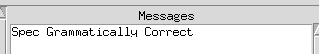
\includegraphics[scale=0.5]{Figures/zcga/zcgacorrect.png} 
& 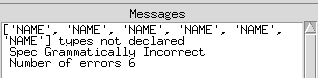
\includegraphics[scale=0.5]{Figures/zcga/zcgaincorrect.png}
\end{tabular}
\caption{Outputting message when specification is correct (left) and incorrect (right).\label{fig:correctandincorrect}}
\end{figure}

In figure \ref{fig:correctandincorrect} the left image shows the outputting message when a specification is \gls{zcga} correct. The right image shows a specification in which a specification is not \gls{zcga} correct as the type `\texttt{NAME}' has been used 6 times in the specification but has not been declared.

\subsection{Errors}
\label{subsec:zcgaerrors}

The specification is \gls{zcga} correct when all labelled objects within the specification follow the \gls{zcga} type rules (table \ref{tab:wttrules}). Here we highlight what error messages one might get when running the \gls{zcga} checker on a specification.


\paragraph{\emph{term not declared}}

This follows the rules for variables in table \ref{tab:wttrules}. The message `\emph{term not declared}' will appear if a term is labelled within the schematext and there hasn't been a declaration defining its type previously. Take a look at the following example fo a specification:

\begin{exam}
\label{Kexam}
\begin{verbatim}
\begin{schema}{K}
\text{\declaration{\term{j}:\expression{\nat}}}
\where
\text{\expression{\term{j} < \term{k}}}
\end{schema}
\end{verbatim}
\end{exam}

In the schematext containing the expression \verb|\term{j} < \term{k}| the term \verb|j| has been previosuly declared with the type \verb|\nat| however the term \verb|k| is labelled and used in the expression however it has not been declared or assigned a type. This will cause the error message \emph{term not declared}.

\paragraph{\emph{set not declared}}

Similar to the previous error message, this follows the rules for variables in table \ref{tab:wttrules}. The message \emph{set not declared} will appear when a variable is labelled \verb|\set{..}| in the schematext of a specifiation but has not been declared previously. Look at the following example:

\begin{exam}
\begin{verbatim}       
\begin{schema}{U}
\text{\declaration{\term{j}:\expression{\nat}}}
\where
\text{\expression{\term{j} \in \set{js}}}
\end{schema}
\end{verbatim}
\end{exam}

When the \gls{zcga} checker runs through this specification the error message \emph{js: set not declared} should appear. This is because the term \verb|j| has been declared, however the set \verb|js| has not been declared yet it is used in the schematext \verb|\term{j} \in \set{js}|.

\paragraph{\emph{constant not in preface}}

When a constant is used within a specification that is not in the preface (see \gls{zcga} code to see all constants in preface) then the `\emph{constant not in preface}' error message will appear. An example is shown in the following specification:

\begin{exam}
\begin{verbatim}       
\begin{schema}{T}
\text{\declaration{\set{t}:\expression{\mathbb{P} \nat}}}
\where
\text{\expression{\set{t} = \set{\{\}}}}
\end{schema}
\end{verbatim}
\end{exam}

The error message will appear here when running the \gls{zcga} checker on the specification as the constant `\verb|\mathbb{P}|' is not in the preface. The user in this case may have meant to use the constant \verb|\power| instead of \verb|\mathbb{P}|. Even though these two constants look identical when compiling a \LaTeX{} document they are not the same when checking specifications with \gls{zcga}.

\paragraph{\emph{constant already in specification}}

The error message \emph{constant already in specification} will appear if the user tries to define a constant which is already in the preface constants or defined constants. For example take a look at the following specification:

\begin{exam}
\begin{verbatim}
\set{\nat} := \term{1} | \term{2} | \term{3} |...
\end{verbatim}
\end{exam}

The \gls{zcga} would say this specification is incorrect and the error `\emph{constant already in specification}' would appear as the user is trying to define the set of natural numbers \verb|\nat| however this constant is already programmed in the preface of constants for Z specifications.

This error would also appear if the user tried to define a constant such as \verb|[STUDETS]| more  than once in their specification.

\paragraph{\emph{not a correct term}}

For this error message to appear, the user must have tried to create a term when it wasn't allowed. Take the following example:

\begin{exam}
\begin{verbatim}       
\begin{schema}{Y}
\text{\declaration{\term{y}:\expression{\nat}}}
\where
\text{\expression{\term{\# \term{y}} = \term{0}}}
\end{schema}
\end{verbatim}
\end{exam}

This specification would be \gls{zcga} incorrect and the error message \emph{not a correct term} would appear due to the term \verb|\term{\# \term{y}}| being incorrect. This is because the constant \verb|\#| takes a set as a parameter and gives back a term (the cardinality of the set). In this case the user has applied a term \verb|\term{y}| to the constant \verb|\#| and thus the error message appearing.

\paragraph{\emph{not a correct set}}

The error message \emph{not a correct set} will appear when a user has labelled something as a set when it is not. For example take the following specification:

\begin{exam}
\begin{verbatim}       
\begin{schema}{W}
\text{\declaration{\term{w}:\expression{\power \nat}}}
\text{\declaration{\term{w'}:\expression{\power \nat}}}
\text{\declaration{\term{v}:\expression{\nat}}}
\where
\text{\expression{\set{w'} = \set{\set{w} \cup \term{v}}}}
\end{schema}
\end{verbatim}
\end{exam}

In this case the incorrect set would be \verb|\set{\set{w} \cup \term{v}}|. This is because the constant \verb|\cup| takes two sets as parameters. However this labelling shows that a set `\verb|w|' and a term `\verb|v|' have been applied. 

%If the user wished to ammend this then the set would change to \verb|\set{\set{w} \cup \set{\{\term{v}\}}}|. By adding the curly brackets \verb|\{..\}| it changes the term into a set which can now be applied as a parameter to \verb|\cup|.

\section{Benefits}

In addition to the main use for the \gls{zcga} checker which is to check the grammar of a formal specification written in Z other benefits exists. The \gls{zcga} would also be an advantage to the user or designer of a system to translate their ideas to the developers of the system. For example by using the \gls{zcga} the developers can clearly see which parts of the systems are represented as sets and which parts are represented as terms. Not only does it help describe the system to developers but other memebers of the project development team and other stakeholders such as the client would also get a better idea of the layout of the system.
A further advantage to the \gls{zcga} is that it is able to check the grammatical correctness of partially-formal specifications. These can include specifications written in the english natural langugage but are on their way to becoming formal, or specifications with formal parts to them.

\section{Conclusion}
In this chapter we have seen how the \gls{zcga} has grown from weak type theory for mathematics \cite{wtt}. We have giving examples of different categories are used within a Z specification and highlighted the rules these categories need to follow in order to be \gls{zcga} correct. We have described a few properties of the checker and have explained how these categories are transformed into weak types for Z. We explained how a Z specification can be annotated and checked bu the \gls{zcga} and given and illustrated the different errors which may arise. The next step of the \gls{zmath} framework to check for another type of correctness, the \gls{zdra}.
